%!TEX root = ../Thesis.tex
\chapter{Kalman Filtering}

\section{Theory Derivation}
\label{sec:kalman_theory}

The Kalman filter is used to estimate the internal state of a stochastic
system from noisy measurements. The system considered in this work is

\begin{align}
    x_{t+1} &= Ax_t + Bu_t + w_t \\
    y_t &= Cx_t + v_t
\end{align}

where

\begin{equation}
    w_t \sim \mathcal{N}(0,R_w),
    \qquad
    v_t \sim \mathcal{N}(0,R_v)
\end{equation}

Let

\begin{equation}
    Y_t = \{y_0,\ldots,y_t\}
\end{equation}

denote all measurements available up to time \(t\). Before receiving the
measurement \(y_t\), the state distribution conditioned on the previous
measurements is represented by

\begin{equation}
    x_t \mid Y_{t-1}
    \sim
    \mathcal{N}
    \left(
        \hat{x}_{t|t-1},
        P_{t|t-1}
    \right)
\end{equation}

Thus, before \(y_t\) is observed, the best available state estimate is
\(\hat{x}_{t|t-1}\), with uncertainty represented by \(P_{t|t-1}\).

To incorporate the new measurement, the joint distribution of the state and
measurement is considered. Since the system and noise distributions are
Gaussian, the variables \(x_t\) and \(y_t\), conditioned on the previous
measurements, are jointly Gaussian.

The required moments are first derived. The conditional mean of the state is

\begin{equation}
    E[x_t \mid Y_{t-1}]
    =
    \hat{x}_{t|t-1}
\end{equation}

The conditional mean of the measurement becomes

\begin{align}
    E[y_t \mid Y_{t-1}]
    &=
    E[Cx_t+v_t \mid Y_{t-1}] \\
    &=
    C E[x_t \mid Y_{t-1}] \\
    &=
    C\hat{x}_{t|t-1}
\end{align}

The covariance between the measurement and the state is

\begin{align}
    \operatorname{Cov}
    (y_t,x_t \mid Y_{t-1})
    &=
    \operatorname{Cov}
    (Cx_t+v_t,x_t \mid Y_{t-1}) \\
    &=
    C\operatorname{Cov}
    (x_t,x_t \mid Y_{t-1}) \\
    &=
    CP_{t|t-1}
\end{align}

Similarly,

\begin{equation}
    P_{xy}
    =
    P_{yx}^{T}
    =
    P_{t|t-1}C^T
\end{equation}

The measurement covariance is

\begin{align}
    \operatorname{Cov}
    (y_t \mid Y_{t-1})
    &=
    \operatorname{Cov}
    (Cx_t+v_t,Cx_t+v_t \mid Y_{t-1}) \\
    &=
    CP_{t|t-1}C^T+R_v
\end{align}

Therefore,

\begin{equation}
\begin{bmatrix}
    x_t \\
    y_t
\end{bmatrix}
\Bigg|
Y_{t-1}
\sim
\mathcal{N}
\left(
\begin{bmatrix}
    \hat{x}_{t|t-1} \\
    C\hat{x}_{t|t-1}
\end{bmatrix},
\begin{bmatrix}
    P_{t|t-1}
    &
    P_{t|t-1}C^T
    \\
    CP_{t|t-1}
    &
    CP_{t|t-1}C^T+R_v
\end{bmatrix}
\right)
\end{equation}

The measurement update can then be obtained using the projection theorem.

For two jointly Gaussian variables,

\begin{equation}
    Z=
    \begin{bmatrix}
        X \\
        Y
    \end{bmatrix}
    \sim
    \mathcal{N}
    \left(
    \begin{bmatrix}
        m_x \\
        m_y
    \end{bmatrix},
    \begin{bmatrix}
        P_x & P_{xy} \\
        P_{xy}^T & P_y
    \end{bmatrix}
    \right)
\end{equation}

the conditional distribution is

\begin{equation}
    X|Y
    \sim
    \mathcal{N}
    \left(
        m_x
        +
        P_{xy}P_y^{-1}(y-m_y),
        \;
        P_x
        -
        P_{xy}P_y^{-1}P_{xy}^T
    \right)
\end{equation}

The projection theorem therefore provides the conditional mean and covariance
of the state after the measurement has been observed. Applying it to the
joint distribution of \(x_t\) and \(y_t\) gives the measurement-update
equations

\begin{equation}
    \boxed{
    \hat{x}_{t|t}
    =
    \hat{x}_{t|t-1}
    +
    P_{t|t-1}C^T
    \left(
        CP_{t|t-1}C^T+R_v
    \right)^{-1}
    \left(
        y_t-C\hat{x}_{t|t-1}
    \right)
    }
\end{equation}

and

\begin{equation}
    \boxed{
    P_{t|t}
    =
    P_{t|t-1}
    -
    P_{t|t-1}C^T
    \left(
        CP_{t|t-1}C^T+R_v
    \right)^{-1}
    CP_{t|t-1}
    }
\end{equation}

After the measurement update, the state estimate is propagated to the next
time step. From the system dynamics,

\begin{equation}
    x_{t+1}
    =
    Ax_t+Bu_t+w_t,
\end{equation}

the predicted state estimate becomes

\begin{equation}
    \boxed{
    \hat{x}_{t+1|t}
    =
    A\hat{x}_{t|t}+Bu_t
    }
\end{equation}

The corresponding covariance is

\begin{equation}
    P_{t+1|t}
    =
    \operatorname{Cov}
    (Ax_t+Bu_t+w_t \mid Y_t),
\end{equation}

which gives

\begin{equation}
    \boxed{
    P_{t+1|t}
    =
    AP_{t|t}A^T+R_w
    }
\end{equation}

The predicted quantities at time \(t+1\) then become the prior quantities for
the next iteration, and the procedure is repeated when the next measurement
is received.


\subsection{Overview}
\label{subsec:kalman_overview}

The Kalman filter therefore consists of two main stages: the measurement
update and the time update.

Starting with the prior state estimate

\begin{equation}
    \hat{x}_{k|k-1},
    \qquad
    P_{k|k-1}
\end{equation}

the current measurement \(y_k\) is first used to obtain the posterior state
estimate

\begin{equation}
    \hat{x}_{k|k}
    =
    \hat{x}_{k|k-1}
    +
    P_{k|k-1}C^T
    \left(
        CP_{k|k-1}C^T+R_v
    \right)^{-1}
    \left(
        y_k-C\hat{x}_{k|k-1}
    \right)
\end{equation}

with covariance

\begin{equation}
    P_{k|k}
    =
    P_{k|k-1}
    -
    P_{k|k-1}C^T
    \left(
        CP_{k|k-1}C^T+R_v
    \right)^{-1}
    CP_{k|k-1}
\end{equation}

This corresponds to the measurement update.

The resulting posterior state estimate is then propagated forward through the
system model according to

\begin{equation}
    \hat{x}_{k+1|k}
    =
    A\hat{x}_{k|k}
    +
    Bu_k
\end{equation}

and

\begin{equation}
    P_{k+1|k}
    =
    AP_{k|k}A^T+R_w
\end{equation}

This corresponds to the time update. The predicted state
\(\hat{x}_{k+1|k}\) then becomes the prior estimate for the next measurement
step \(\hat{x}_{k|k-1}\), and the same procedure is repeated.



\section{Results}
\label{sec:kalman_results}

The Kalman filter was evaluated using the stochastic bilinear system employed
in the previous chapter. The system matrices were

\begin{equation}
    A(v)
    =
    \begin{bmatrix}
        0.90 & v \\
        0.00 & 0.50
    \end{bmatrix},
    \qquad
    B(v)
    =
    \begin{bmatrix}
        0 \\
        1
    \end{bmatrix}
\end{equation}

with

\begin{equation}
    C=
    \begin{bmatrix}
        1 & 0
    \end{bmatrix}
\end{equation}

The process and measurement noise covariance matrices were selected as

\begin{equation}
    R_w=
    \begin{bmatrix}
        0.05 & 0 \\
        0 & 0.05
    \end{bmatrix},
    \qquad
    R_v=
    \begin{bmatrix}
        0.005
    \end{bmatrix}
\end{equation}

The initial state distribution was defined using

\begin{equation}
    \mu_0=
    \begin{bmatrix}
        0 \\
        0
    \end{bmatrix},
    \qquad
    P_0=
    \begin{bmatrix}
        0.01 & 0 \\
        0 & 0.01
    \end{bmatrix}
\end{equation}

The controller weighting matrices were selected as

\begin{equation}
    Q=1,
    \qquad
    R_U=0.1,
    \qquad
    R_V=0.1
\end{equation}

and the optimization variables were constrained by

\begin{equation}
    -5\leq u_k\leq5,
    \qquad
    -5\leq v_k\leq5
\end{equation}

The reference levels were \(3.1\) and \(-1.3\), with the reference changing
after 15 time steps.


\subsection{Open-Loop}
\label{subsec:kalman_open_loop}

For the open-loop evaluation, the stochastic bilinear system was simulated
over a horizon of 30 steps using 100 Monte Carlo realizations. The same
optimized \(U\) and \(V\) sequences were used for all Monte Carlo
realizations. The Kalman filter was then applied to the resulting noisy
measurements.

\newpage
\subsubsection{Single Trajectory}

A single Monte Carlo realization was first selected to illustrate the
estimation behavior of the Kalman filter. The estimated states were compared
directly with the corresponding true states.

The uncertainty associated with the state estimate is also shown using the
\(\pm2\sigma\) interval obtained from the posterior covariance matrix. This
provides a visual indication of the uncertainty represented by the filter.

\begin{figure}[H]
    \centering
    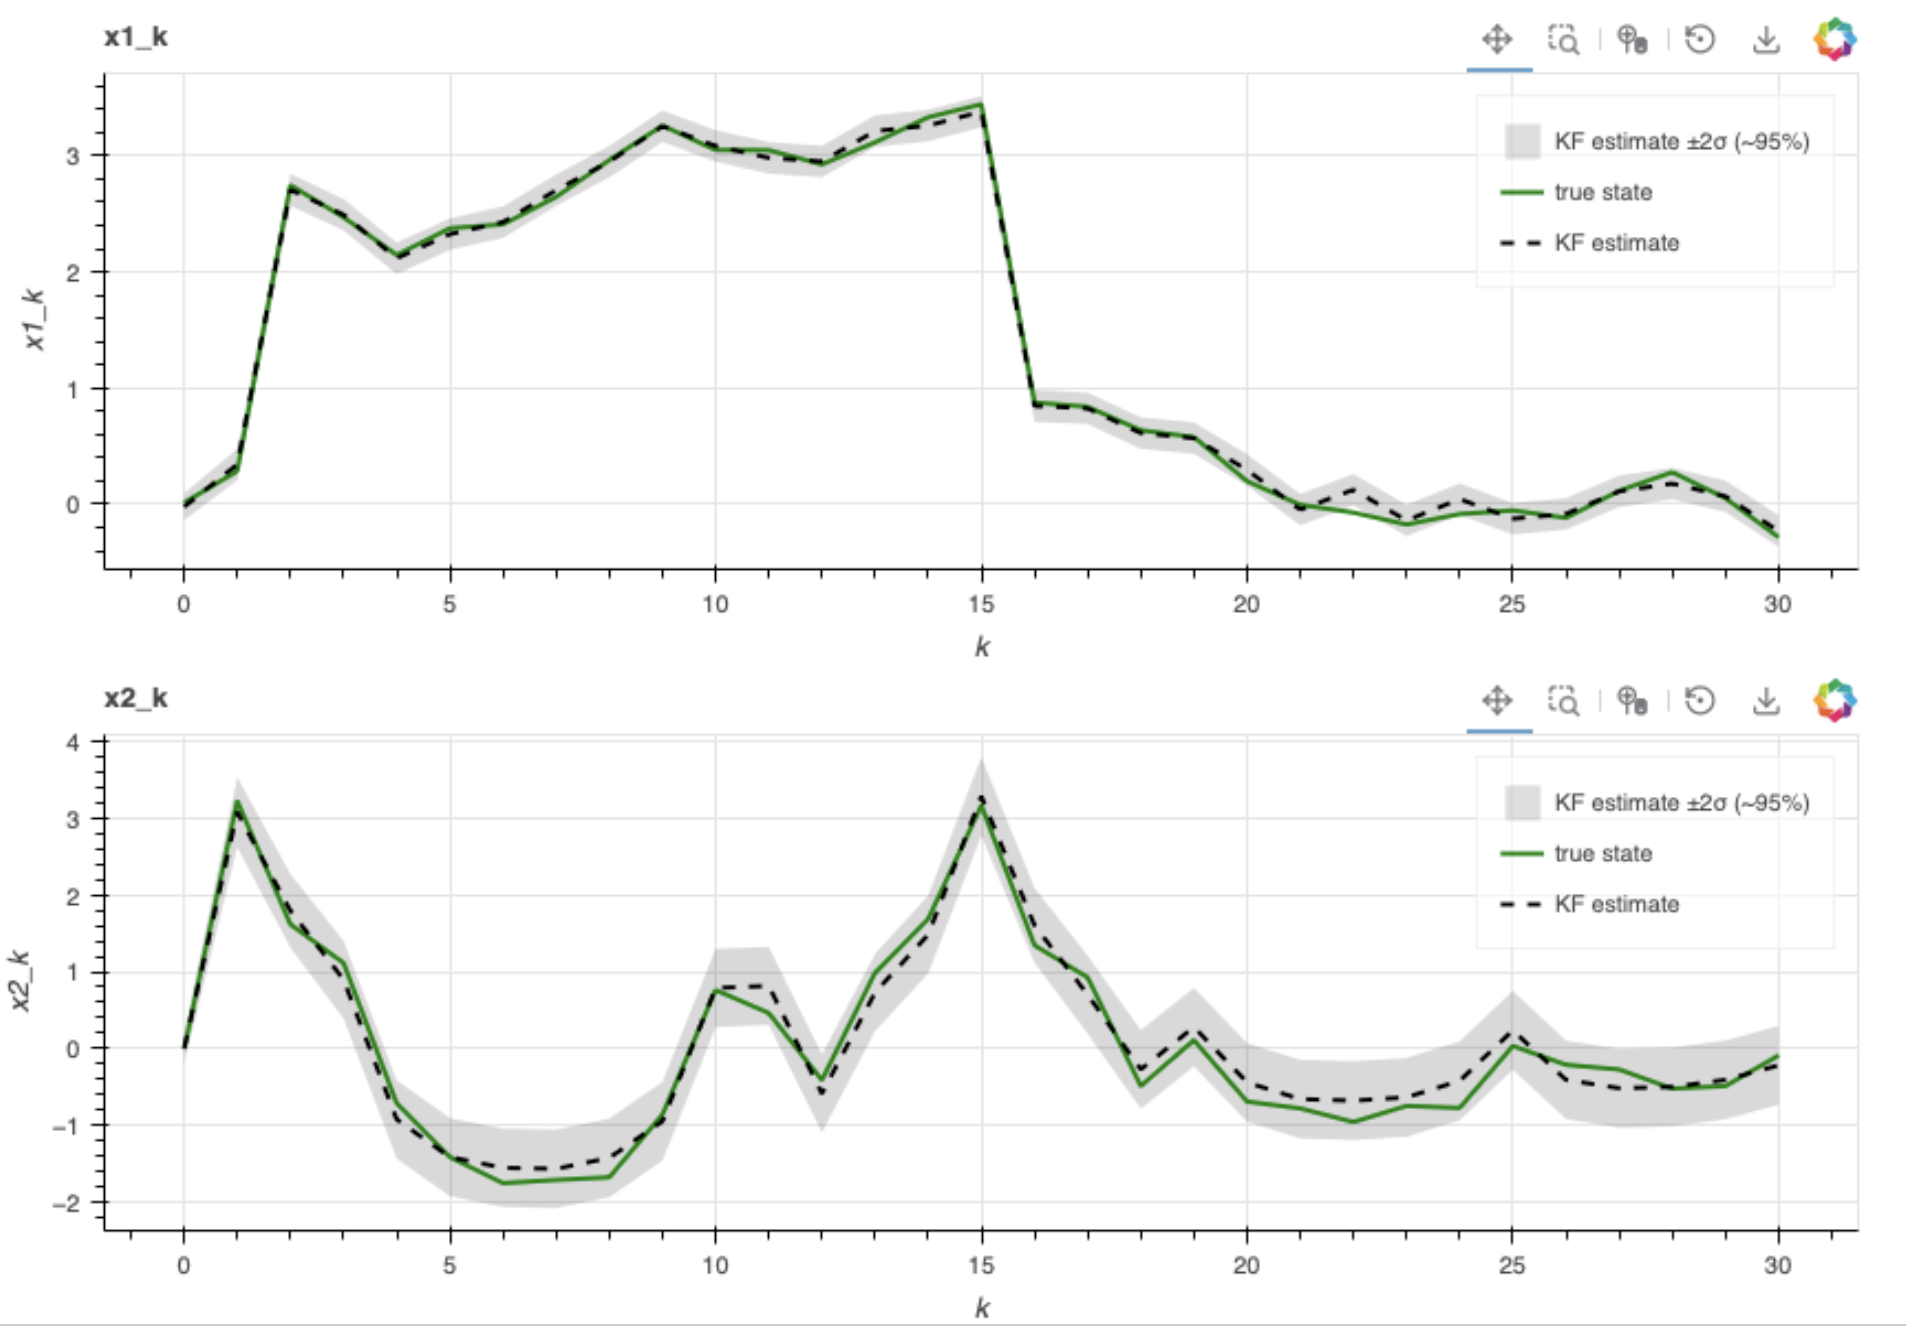
\includegraphics[width=0.9\textwidth]{graphics/kalman_open_single.png}
    \caption{Kalman-filter state estimate for a single stochastic bilinear
    open-loop trajectory}
    \label{fig:kf_bilinear_estimate_openloop}
\end{figure}

\newpage
\subsubsection{Monte Carlo Result}

The Kalman filter was then applied to all Monte Carlo trajectories. The true
state trajectories and their corresponding Kalman-filter estimates are shown
together in order to examine the estimation behavior over repeated stochastic
realizations.

The empirical mean of the true trajectories and the empirical mean of the
estimated trajectories are also displayed. In addition, the corresponding
\(\pm2\sigma\) regions show the spread of the Monte Carlo trajectories.

\begin{figure}[H]
    \centering
    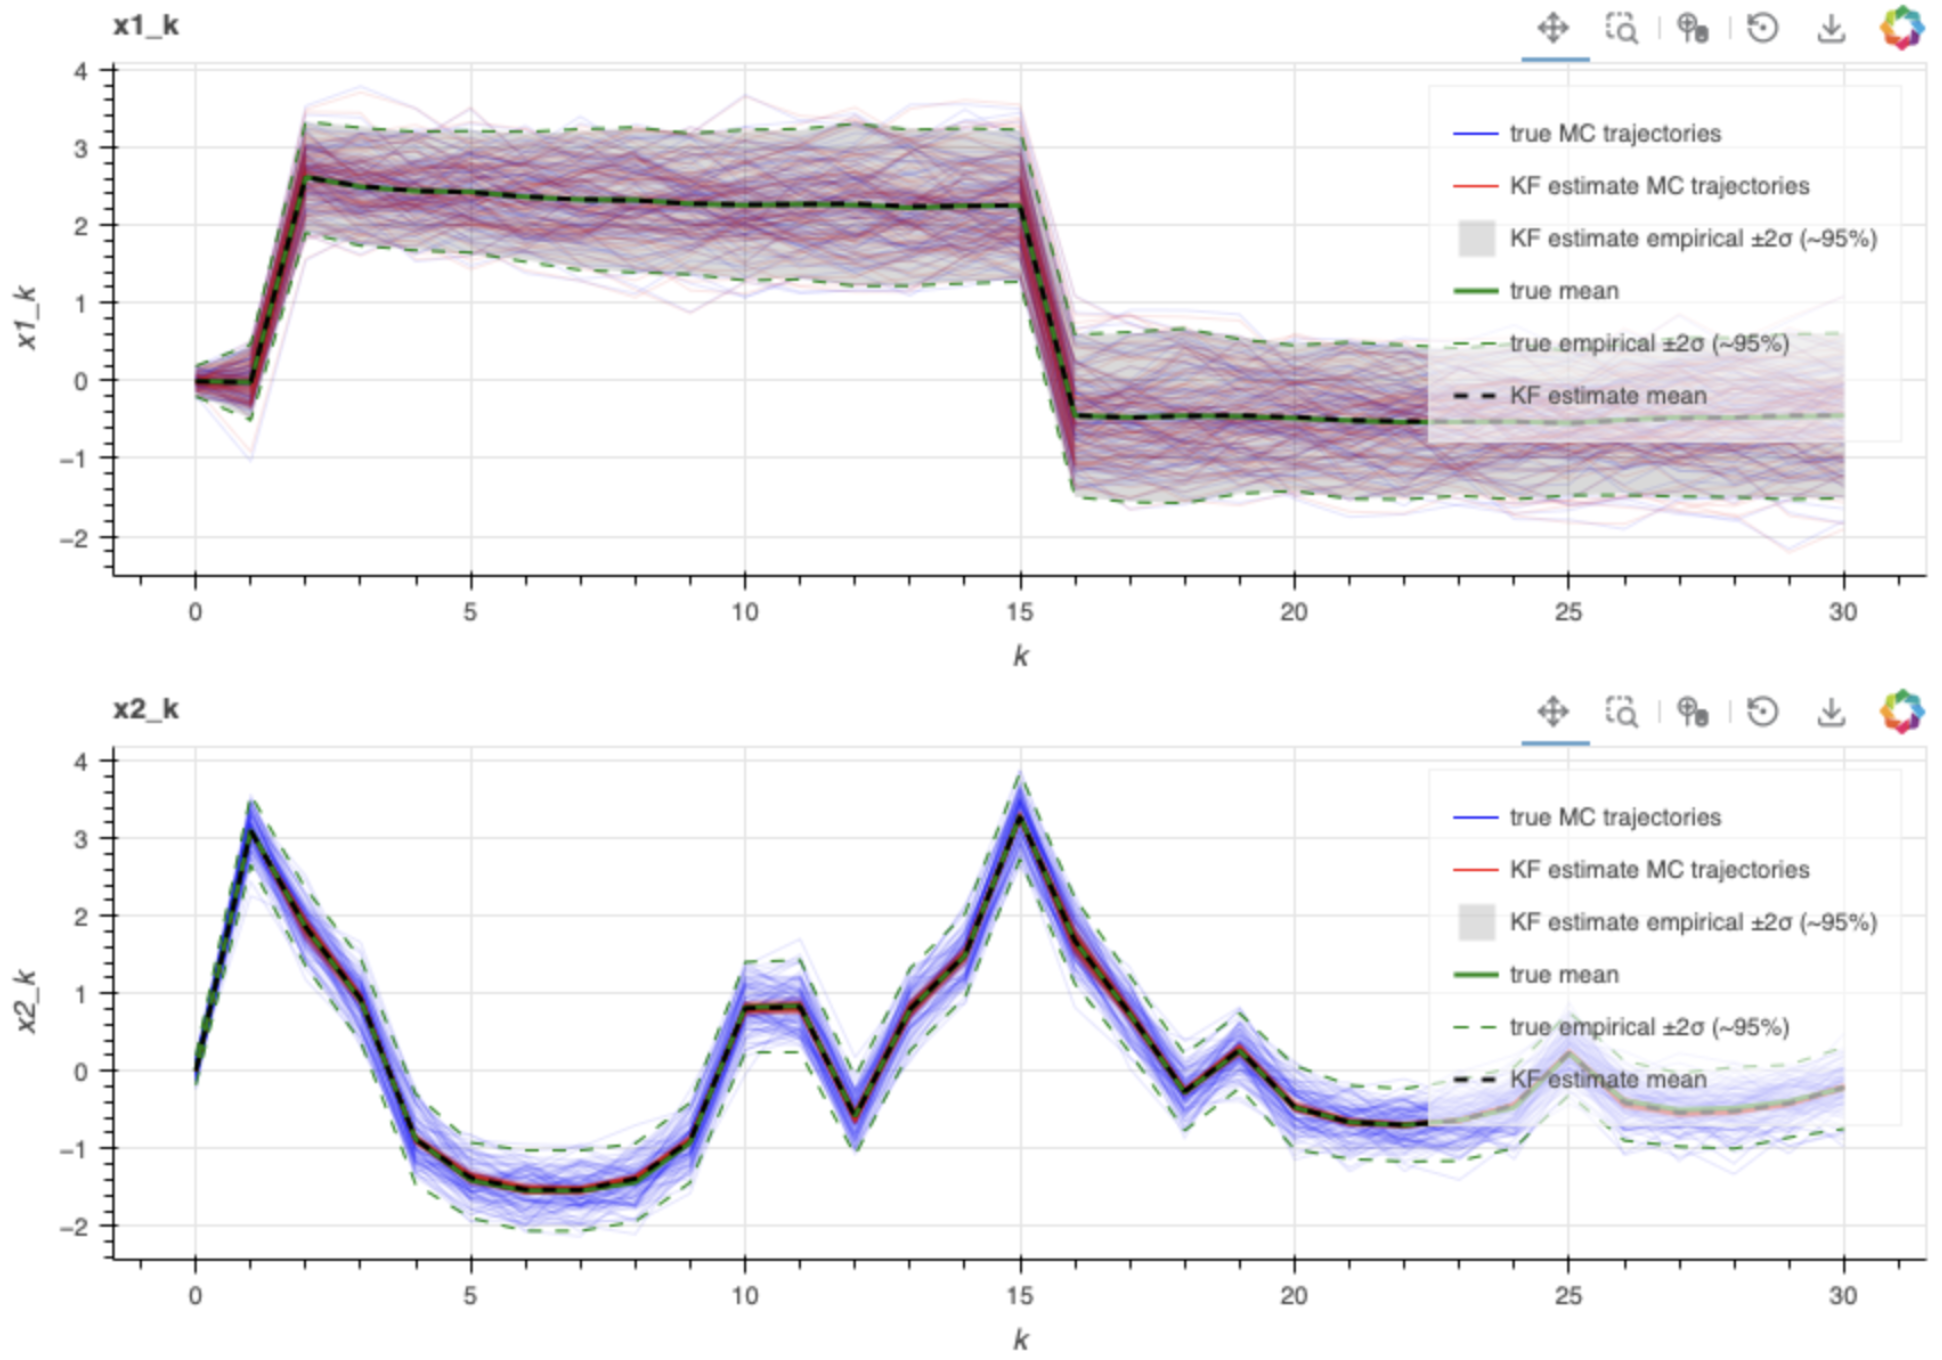
\includegraphics[width=0.9\textwidth]{graphics/kalman_open_multiple.png}
    \caption{Monte Carlo true-state trajectories and Kalman-filter estimates
    for the stochastic bilinear open-loop simulation}
    \label{fig:kf_bilinear_mc_openloop_paths}
\end{figure}

\newpage
\subsubsection{Performance Evaluation}

The performance of the Kalman filter was further evaluated by examining the
difference between the estimated and true states over all Monte Carlo
realizations.

The mean estimation error is shown together with the empirical
\(\pm2\sigma\) spread of the estimation error. This is compared with the
uncertainty predicted by the Kalman covariance matrix.

This comparison provides an indication of whether the covariance calculated
by the Kalman filter appropriately represents the observed estimation
uncertainty over the Monte Carlo simulations.

\begin{figure}[H]
    \centering
    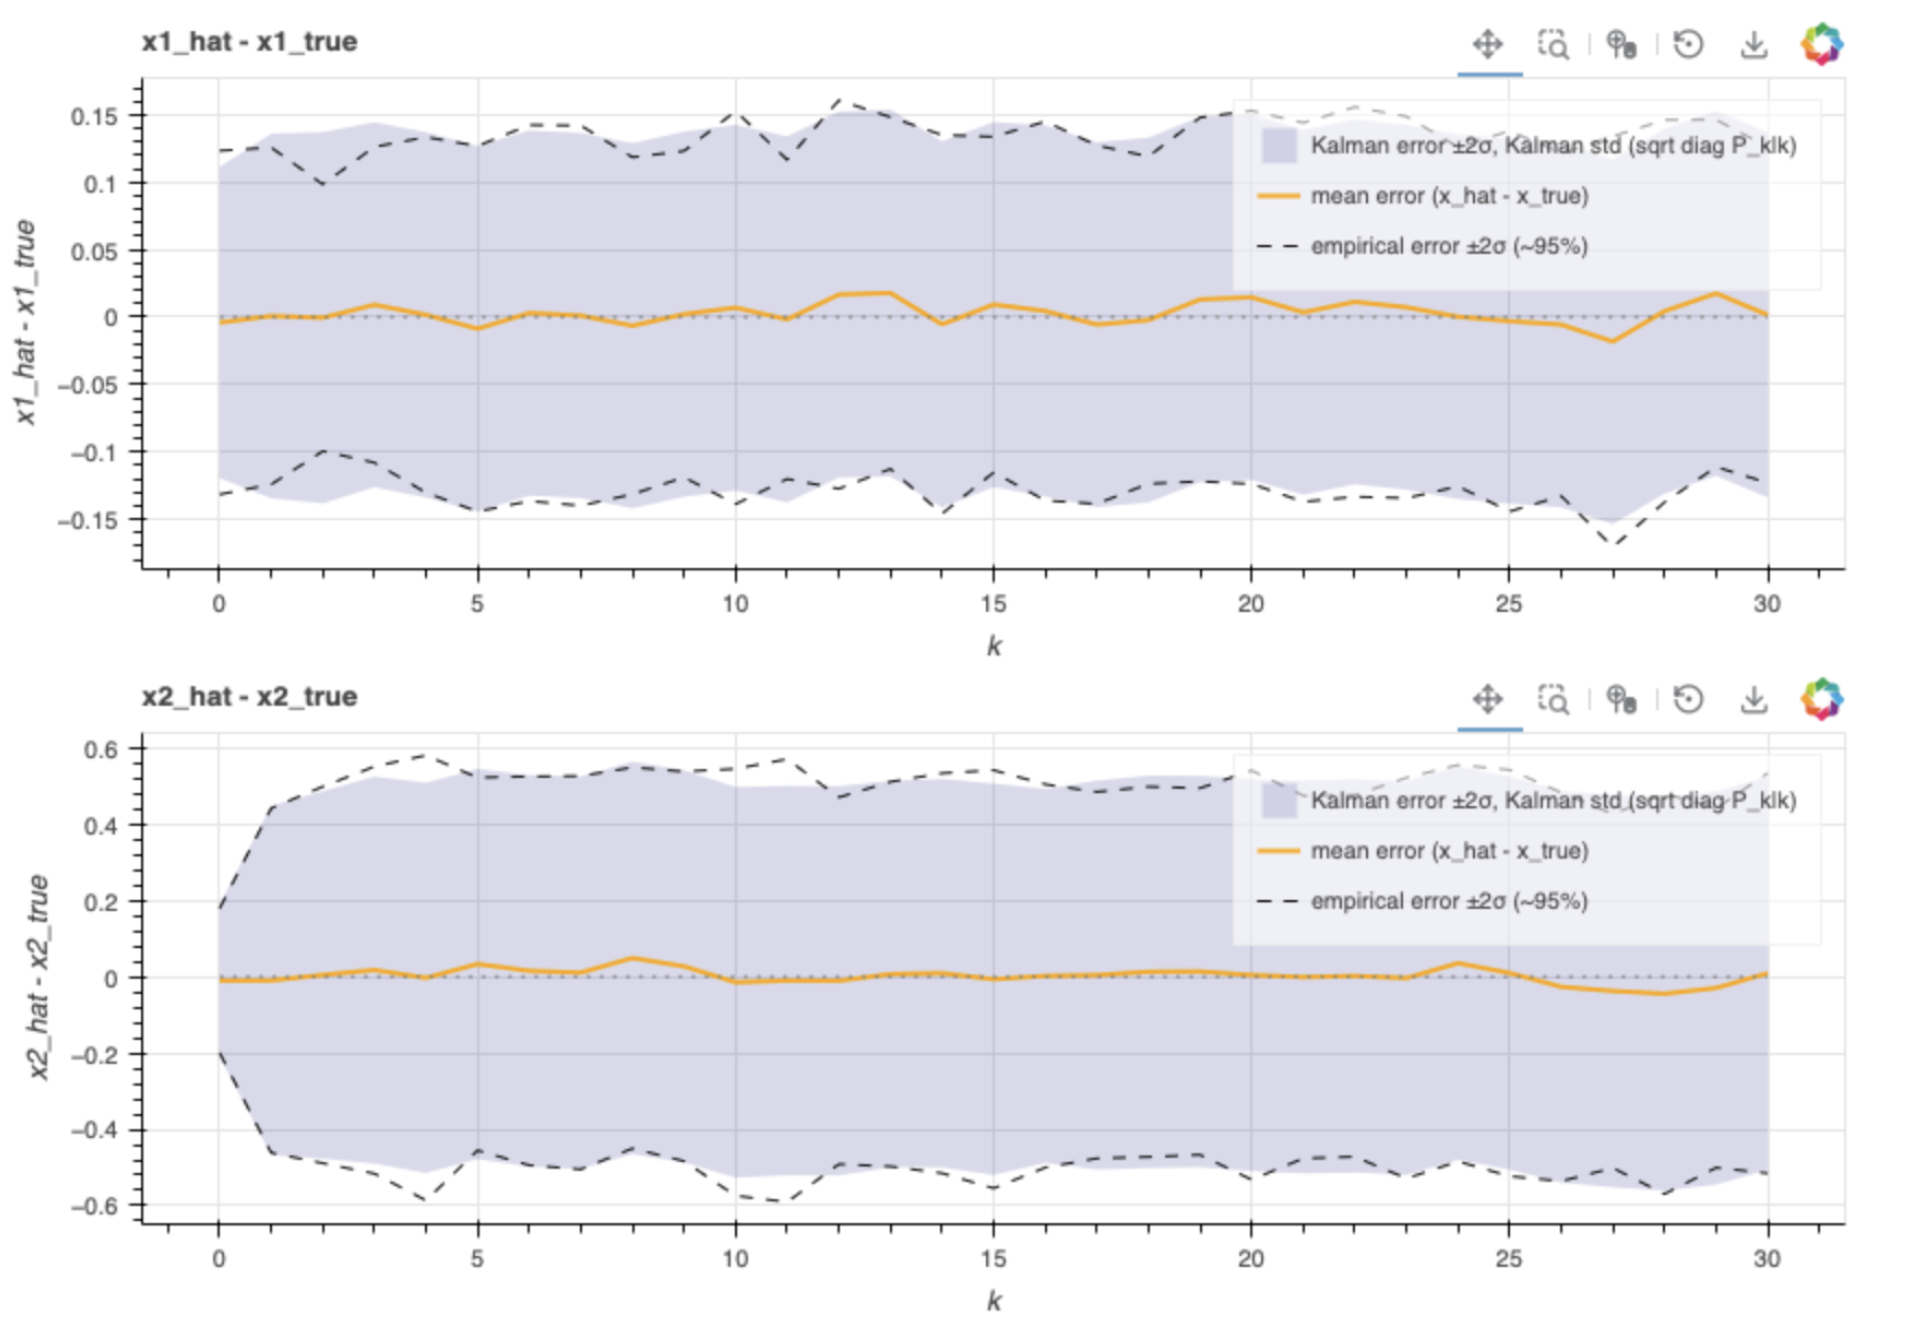
\includegraphics[width=0.9\textwidth]{graphics/kalman_open_performance.png}
    \caption{Mean estimation error and comparison between the empirical and
    Kalman-filter uncertainty for the stochastic bilinear open-loop
    simulation}
    \label{fig:kf_bilinear_mc_openloop_error}
\end{figure}


\subsection{Closed-Loop}
\label{subsec:kalman_closed_loop}

The Kalman filter was also evaluated using the stochastic bilinear
closed-loop simulations. The same system and stochastic parameters were used.

In this case, the input sequences \(U\) and \(V\) can differ between Monte
Carlo realizations. Consequently, the corresponding time-varying system
matrices used in the Kalman-filter prediction step also depend on the
individual realization.

\newpage
\subsubsection{Single Trajectory}

A single closed-loop Monte Carlo realization was first selected. The
Kalman-filter estimate was obtained using the \(U\) and \(V\) sequences
corresponding to that particular trajectory.

The true states, estimated states, and the corresponding \(\pm2\sigma\)
uncertainty interval are shown in
\cref{fig:kf_bilinear_estimate_closedloop}.

\begin{figure}[H]
    \centering
    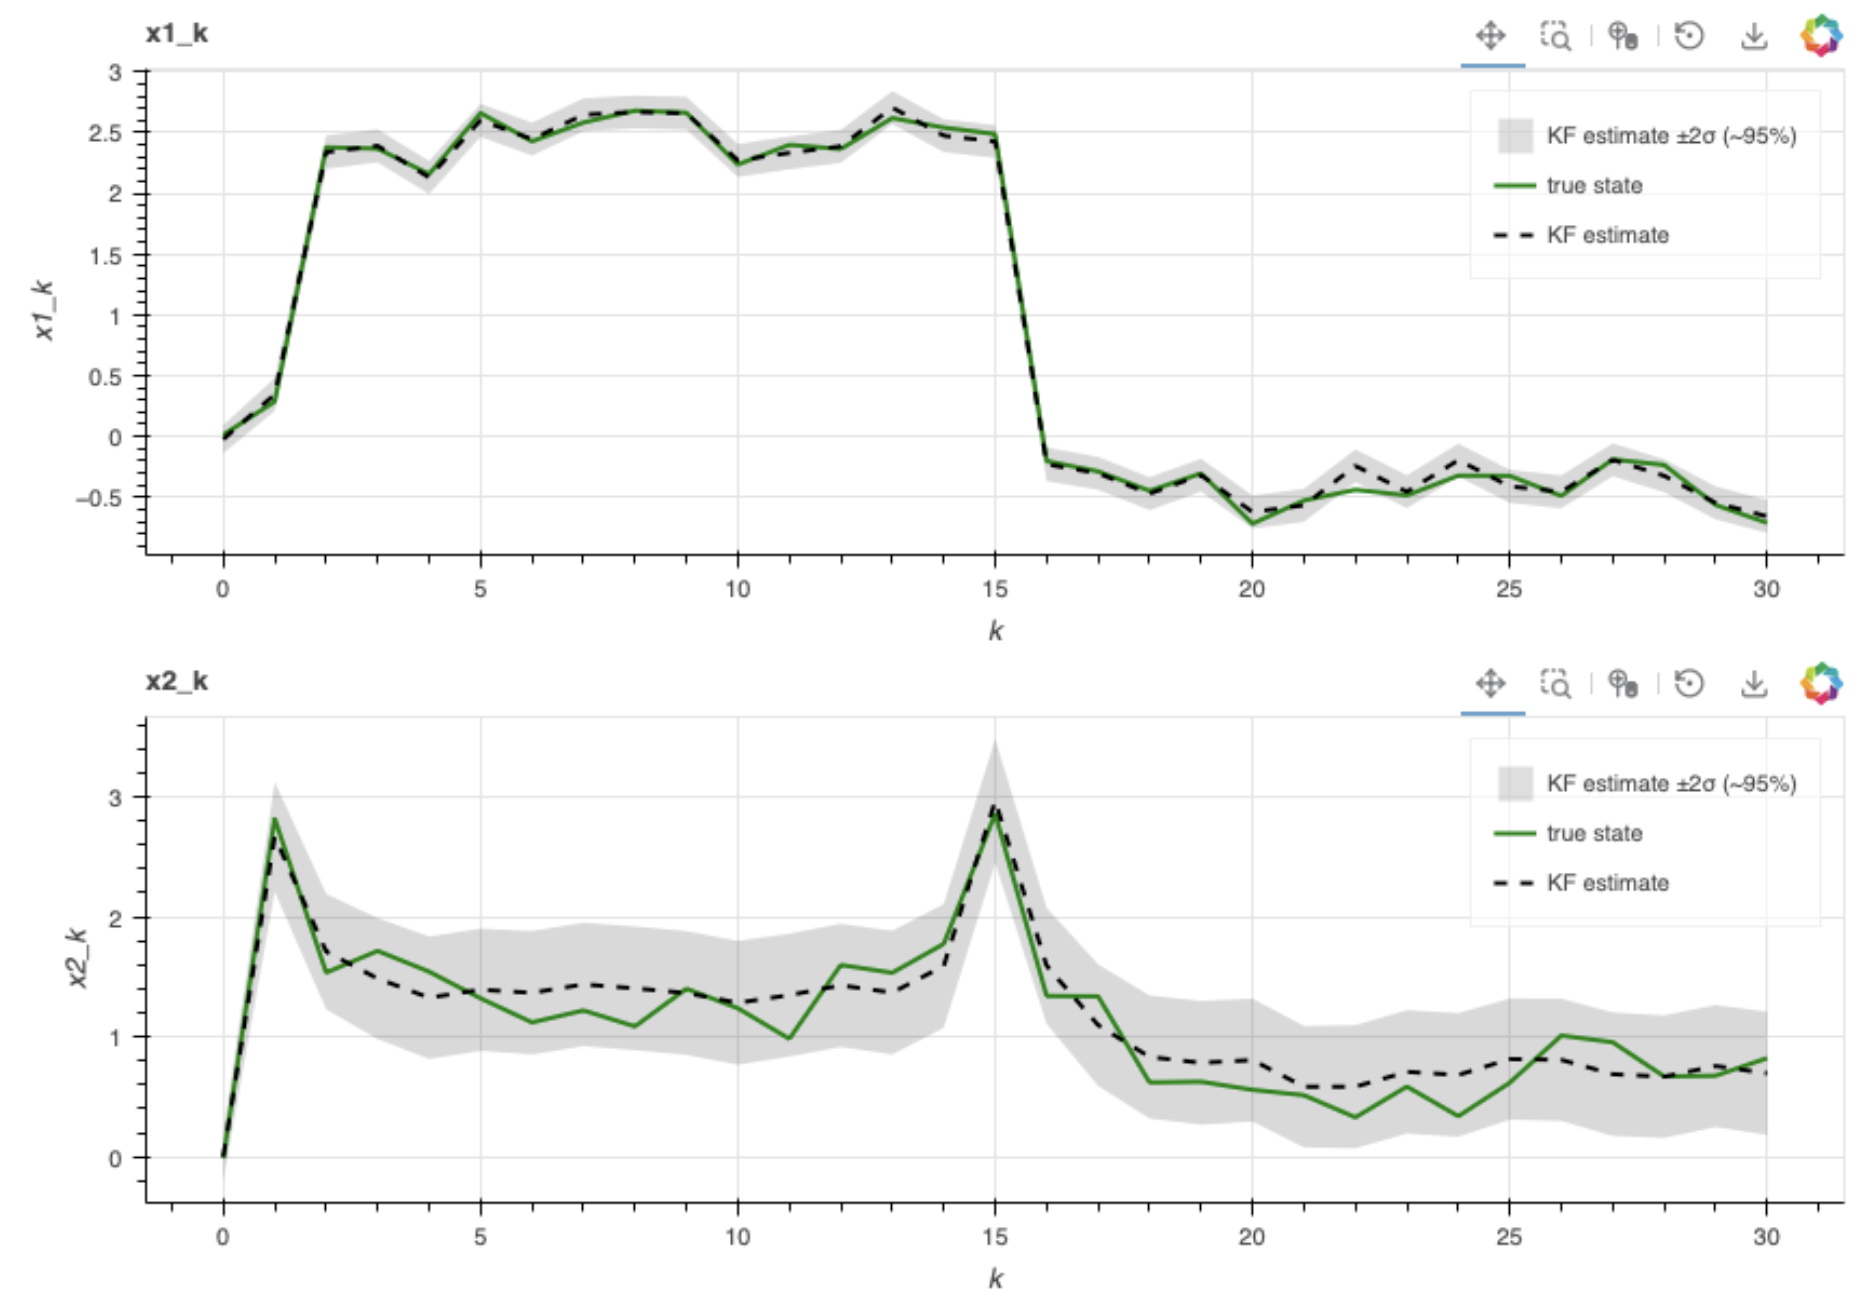
\includegraphics[width=0.9\textwidth]{graphics/kalman_closed_single.png}
    \caption{Kalman-filter state estimate for a single stochastic bilinear
    closed-loop trajectory}
    \label{fig:kf_bilinear_estimate_closedloop}
\end{figure}

\newpage
\subsubsection{Monte Carlo Result}

The filter was subsequently applied to every closed-loop Monte Carlo
trajectory. Since the optimized \(V\)-sequence can differ between
realizations, the corresponding covariance propagation is also evaluated
separately for each trajectory.

The true and estimated state trajectories are shown together with their
empirical means and spreads.

\begin{figure}[H]
    \centering
    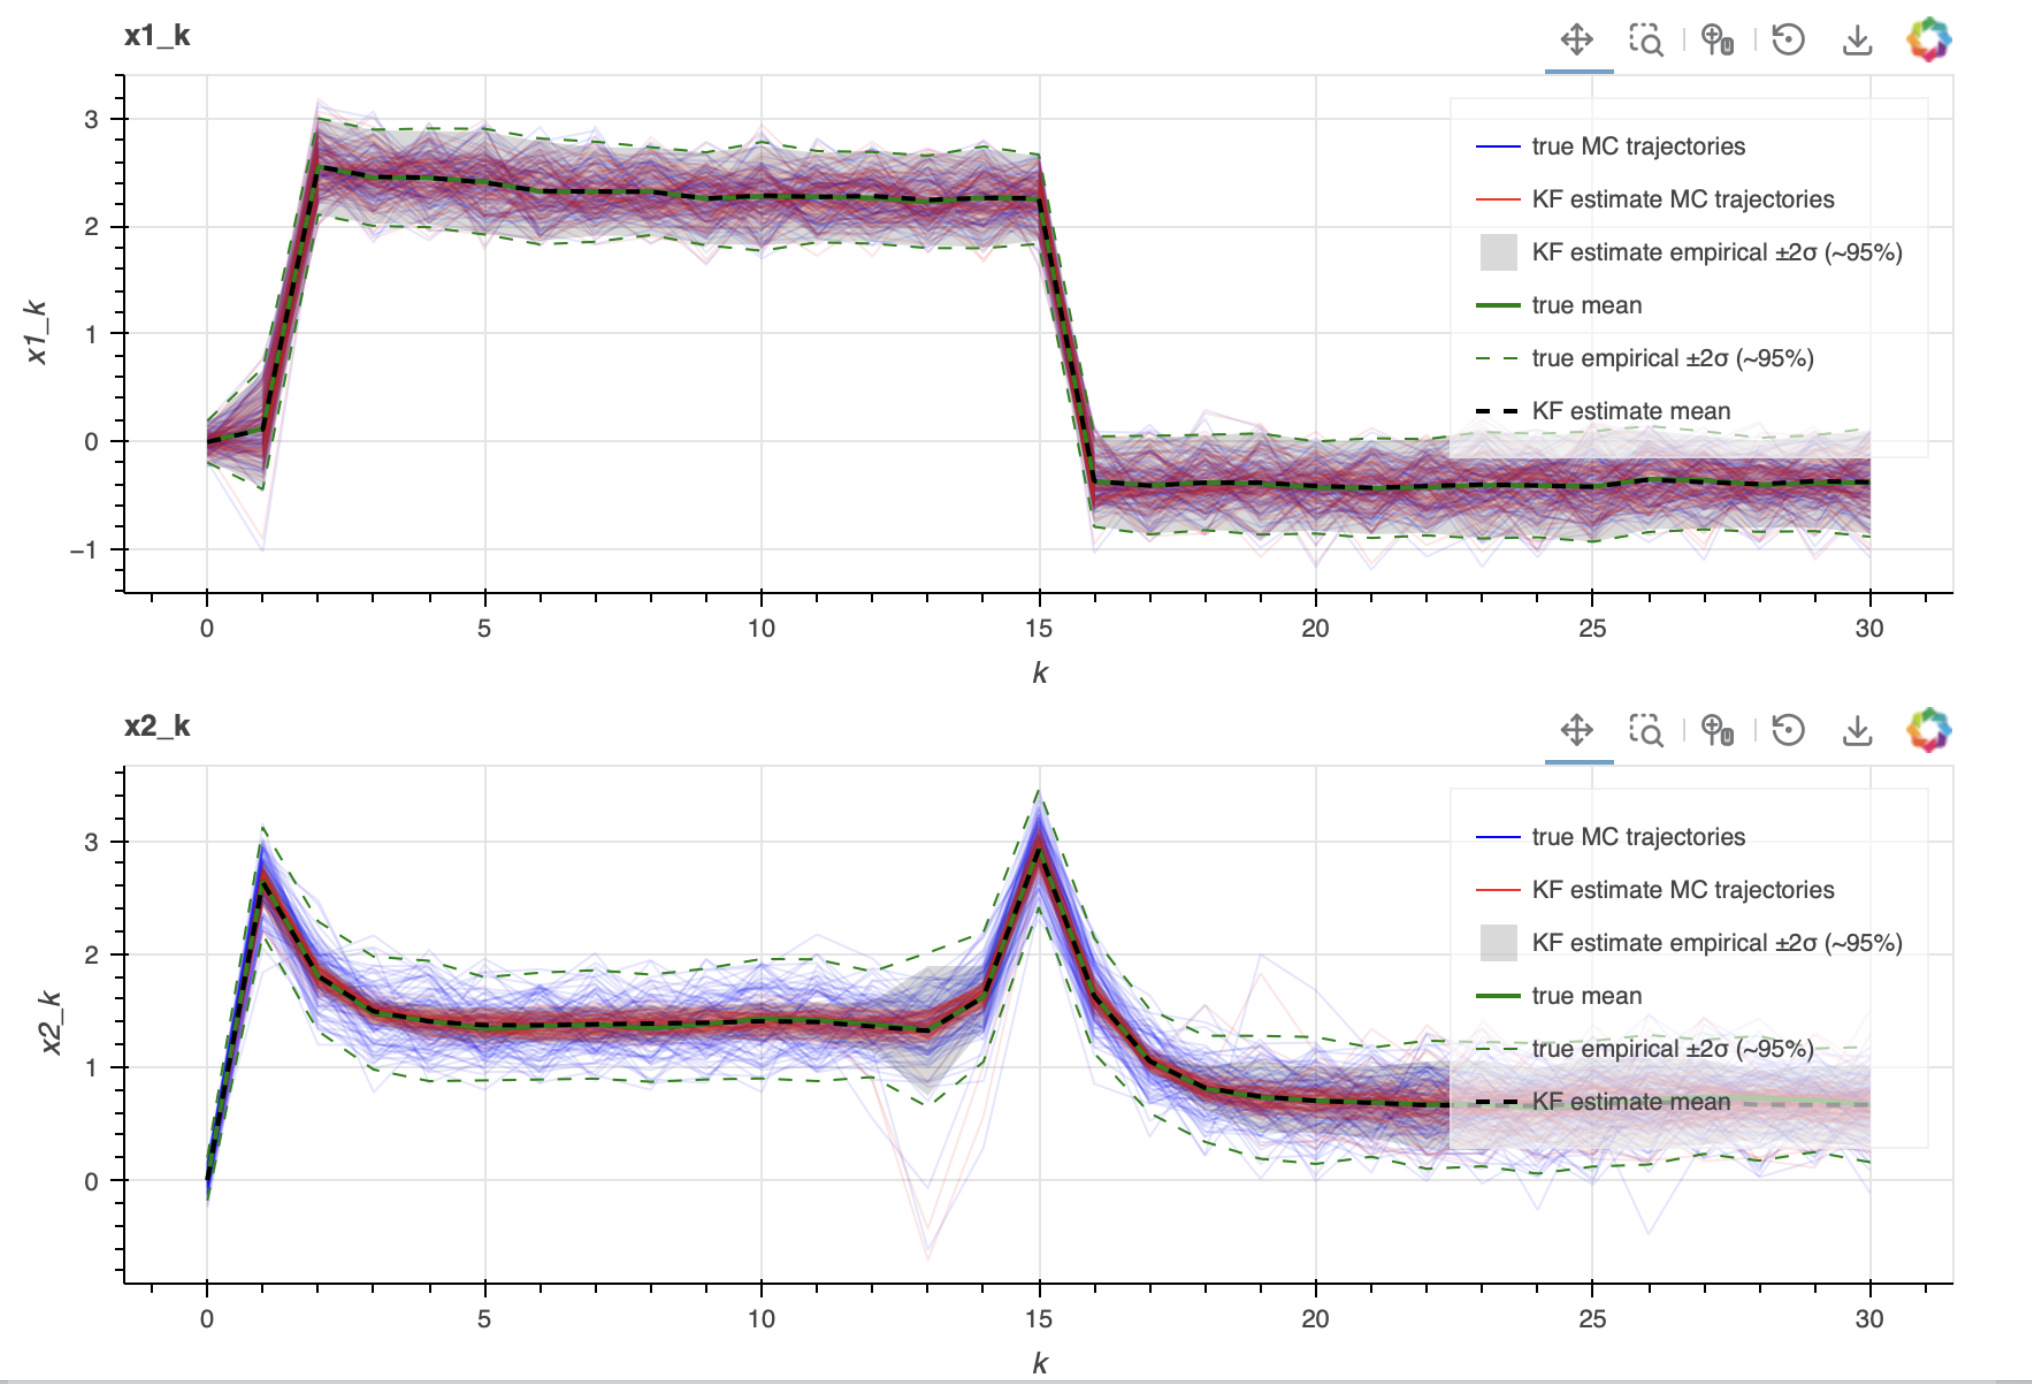
\includegraphics[width=0.9\textwidth]{graphics/kalman_closed_multiple.png}
    \caption{Monte Carlo true-state trajectories and Kalman-filter estimates
    for the stochastic bilinear closed-loop simulation}
    \label{fig:kf_bilinear_mc_closedloop_paths}
\end{figure}

\newpage
\subsubsection{Performance Evaluation}

Finally, the estimation errors from all closed-loop Monte Carlo trajectories
were analyzed.

The mean estimation error and its empirical spread are compared with the
uncertainty obtained from the Kalman covariance matrices. Since each
trajectory may have a different \(V\)-sequence, the covariance evolution can
also differ between simulations.

The comparison therefore provides a statistical evaluation of the state
estimator under the stochastic bilinear closed-loop simulations.

\begin{figure}[H]
    \centering
    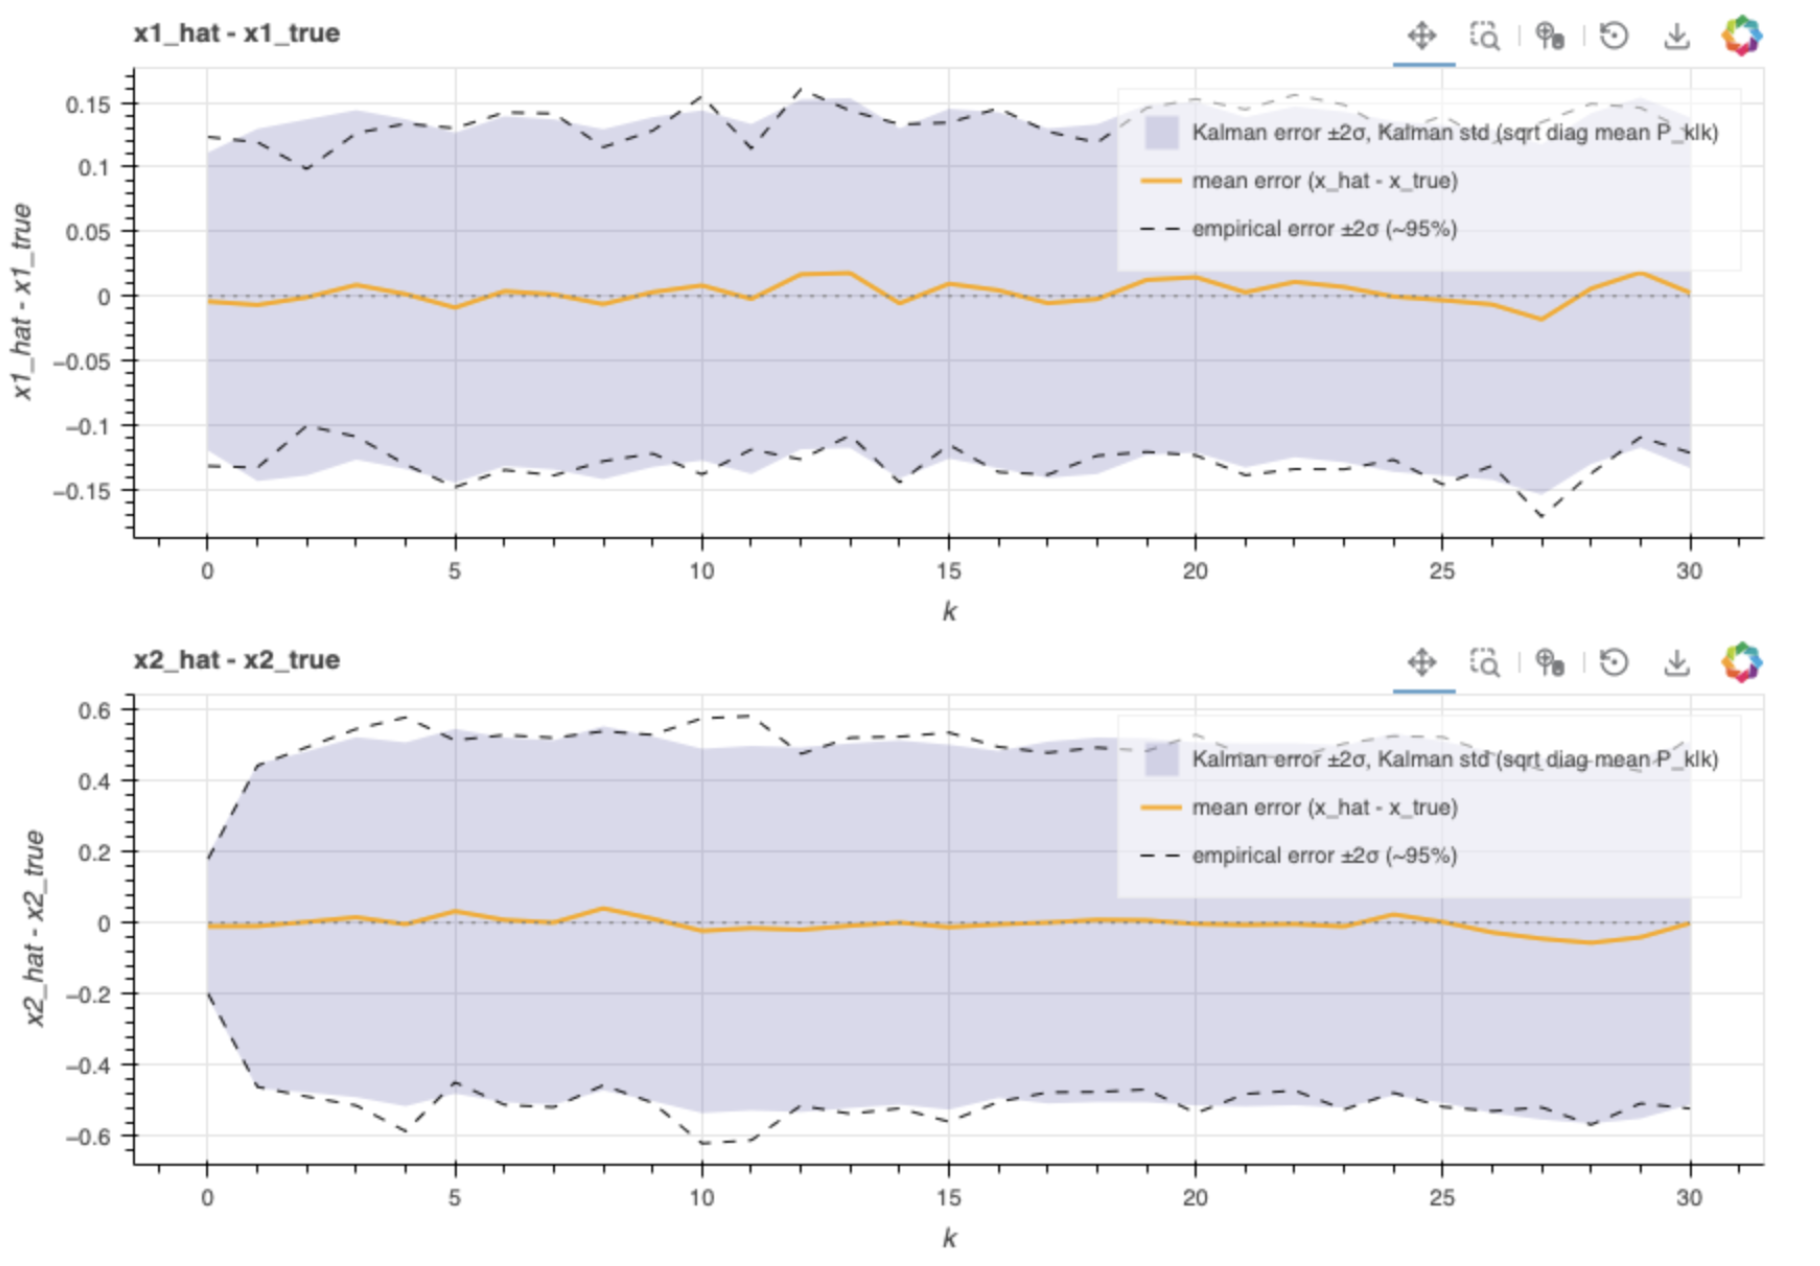
\includegraphics[width=0.9\textwidth]{graphics/kalman_closed_performance.png}
    \caption{Mean estimation error and comparison between the empirical and
    Kalman-filter uncertainty for the stochastic bilinear closed-loop
    simulation}
    \label{fig:kf_bilinear_mc_closedloop_error}
\end{figure}